% ==============================================================================
% BỘ ĐỀ THAM KHẢO TUYỂN SINH 10 NĂM HỌC 2026-2027 SỞ GD&ĐT TP.HCM
% ĐỢT 22: CỤM 15 (ĐỀ 1 & ĐỀ 2 - ĐỀ SỐ 43 VÀ ĐỀ SỐ 44)
% Gồm 14 bài toán tự luận chuẩn cấu trúc tuyển sinh 10
% ==============================================================================

% ==============================================================================
% CỤM 15 - ĐỀ THAM KHẢO 1 (ĐỀ SỐ 43)
% ==============================================================================

\begin{bt}%[9D6H18-2]
% nguon: Đề tham khảo Tuyển sinh 10 năm học 2026-2027 Sở GD&ĐT TP.HCM - Cụm 15 Đề 1 (Đề số 43)
Cho hàm số $y = x^2$ có đồ thị là parabol $(P)$.
\begin{enumerate}[a)]
	\item Vẽ đồ thị $(P)$ trên mặt phẳng toạ độ $Oxy$.
	\item Tìm toạ độ các điểm $M$ thuộc $(P)$ (khác gốc toạ độ $O$) có tung độ gấp $3$ lần hoành độ.
\end{enumerate}
\loigiai{
\begin{enumerate}[a)]
	\item Bảng giá trị tương ứng của $x$ và $y$:
	\begin{center}
		\begin{tabular}{|c|c|c|c|c|c|}
			\hline
			$x$ & $-2$ & $-1$ & $0$ & $1$ & $2$ \\ \hline
			$y = x^2$ & $4$ & $1$ & $0$ & $1$ & $4$ \\ \hline
		\end{tabular}
	\end{center}
	Đồ thị $(P)$ là đường parabol có đỉnh tại gốc toạ độ $O(0;0)$, nhận trục $Oy$ làm trục đối xứng và quay bề lõm lên trên.
	\begin{center}
	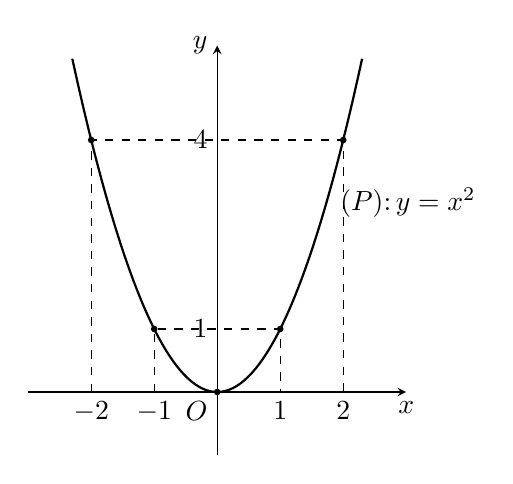
\begin{tikzpicture}[>=stealth,scale=0.8]
		\draw[->] (-3,0) -- (3,0) node[below] {$x$};
		\draw[->] (0,-1) -- (0,5.5) node[left] {$y$};
		\node[below left] at (0,0) {$O$};
		\draw[dashed] (-2,0) node[below] {$-2$} -- (-2,4) -- (0,4) node[left] {$4$} -- (2,4) -- (2,0) node[below] {$2$};
		\draw[dashed] (-1,0) node[below] {$-1$} -- (-1,1) -- (0,1) node[left] {$1$} -- (1,1) -- (1,0) node[below] {$1$};
		\draw[thick,smooth,samples=100,domain=-2.3:2.3] plot(\x,{(\x)^2});
		\fill (-2,4) circle (1.5pt) (-1,1) circle (1.5pt) (0,0) circle (1.5pt) (1,1) circle (1.5pt) (2,4) circle (1.5pt);
		\node[right] at (1.8,3) {$(P)\colon y = x^2$};
	\end{tikzpicture}
	\end{center}
	\item Vì điểm $M$ thuộc $(P)$ có tung độ gấp $3$ lần hoành độ nên ta có $y = 3x$.
	Phương trình hoành độ giao điểm:
	$$x^2 = 3x \iff x^2 - 3x = 0 \iff x(x - 3) = 0 \iff x = 0 \text{ hoặc } x = 3.$$
	Vì điểm $M$ khác gốc toạ độ $O$ nên ta chọn $x = 3 \implies y = 3 \cdot 3 = 9$.
	Vậy toạ độ điểm cần tìm là $M(3; 9)$.
\end{enumerate}
}
\end{bt}

\begin{bt}%[9D6H20-2]
% nguon: Đề tham khảo Tuyển sinh 10 năm học 2026-2027 Sở GD&ĐT TP.HCM - Cụm 15 Đề 1 (Đề số 43)
Cho phương trình $3x^2 - 5x - 7 = 0$.
\begin{enumerate}[a)]
	\item Chứng minh rằng phương trình luôn có hai nghiệm phân biệt $x_1, x_2$.
	\item Không giải phương trình, hãy tính giá trị của biểu thức $A = 4x_1^2 + \dfrac{5x_2}{3} - 5x_1$.
\end{enumerate}
\loigiai{
\begin{enumerate}[a)]
	\item Phương trình $3x^2 - 5x - 7 = 0$ có các hệ số $a = 3$, $b = -5$, $c = -7$.
	Ta có:
	$$\Delta = b^2 - 4ac = (-5)^2 - 4 \cdot 3 \cdot (-7) = 25 + 84 = 109 > 0.$$
	(hoặc do $a \cdot c = 3 \cdot (-7) = -21 < 0$ nên phương trình có hai nghiệm trái dấu).
	Vì $\Delta > 0$ nên phương trình luôn có hai nghiệm phân biệt $x_1, x_2$.
	\item Vì $x_1$ là nghiệm của phương trình nên:
	$$3x_1^2 - 5x_1 - 7 = 0 \implies 3x_1^2 = 5x_1 + 7 \implies x_1^2 = \dfrac{5x_1 + 7}{3}.$$
	Theo định lý Viète, ta có $x_1 + x_2 = -\dfrac{b}{a} = \dfrac{5}{3}$.
	Thay $x_1^2 = \dfrac{5x_1 + 7}{3}$ vào biểu thức $A$, ta được:
	\begin{align*}
		A &= 4 \cdot \dfrac{5x_1 + 7}{3} + \dfrac{5x_2}{3} - 5x_1 \\
		&= \dfrac{20x_1 + 28}{3} + \dfrac{5x_2}{3} - \dfrac{15x_1}{3} \\
		&= \dfrac{20x_1 + 28 + 5x_2 - 15x_1}{3} \\
		&= \dfrac{5x_1 + 5x_2 + 28}{3} \\
		&= \dfrac{5(x_1 + x_2) + 28}{3}.
	\end{align*}
	Thay $x_1 + x_2 = \dfrac{5}{3}$ vào, ta được:
	$$A = \dfrac{5 \cdot \dfrac{5}{3} + 28}{3} = \dfrac{\dfrac{25}{3} + \dfrac{84}{3}}{3} = \dfrac{\dfrac{109}{3}}{3} = \dfrac{109}{9}.$$
	Vậy $A = \dfrac{109}{9}$.
\end{enumerate}
}
\end{bt}

\begin{bt}%[9D8H26-3]
% nguon: Đề tham khảo Tuyển sinh 10 năm học 2026-2027 Sở GD&ĐT TP.HCM - Cụm 15 Đề 1 (Đề số 43)
Biểu đồ cột kép biểu diễn số lượng học sinh tham gia câu lạc bộ cầu lông của một trường THCS như sau:
\begin{center}
\begin{tabular}{|l|c|c|c|c|}
	\hline
	Khối & Khối $6$ & Khối $7$ & Khối $8$ & Khối $9$ \\ \hline
	Nam & $10$ & $12$ & $7$ & $5$ \\ \hline
	Nữ & $8$ & $15$ & $6$ & $7$ \\ \hline
\end{tabular}
\end{center}
Chọn ngẫu nhiên một học sinh tham gia câu lạc bộ cầu lông của trường đó. Tính xác suất của mỗi biến cố sau:
\begin{enumerate}[a)]
	\item $A$: ``Học sinh được chọn là nữ''.
	\item $B$: ``Học sinh được chọn là nam và không thuộc khối $6$''.
\end{enumerate}
\loigiai{
Tổng số học sinh tham gia câu lạc bộ cầu lông của trường là:
$$n(\Omega) = (10 + 8) + (12 + 15) + (7 + 6) + (5 + 7) = 18 + 27 + 13 + 12 = 70\text{ (học sinh)}.$$
\begin{enumerate}[a)]
	\item Tổng số học sinh nữ tham gia câu lạc bộ là:
	$$n(A) = 8 + 15 + 6 + 7 = 36\text{ (học sinh)}.$$
	Xác suất của biến cố $A$ là:
	$$P(A) = \dfrac{n(A)}{n(\Omega)} = \dfrac{36}{70} = \dfrac{18}{35}.$$
	\item Số học sinh nam không thuộc khối $6$ (thuộc khối $7$, $8$, $9$) là:
	$$n(B) = 12 + 7 + 5 = 24\text{ (học sinh)}.$$
	Xác suất của biến cố $B$ là:
	$$P(B) = \dfrac{n(B)}{n(\Omega)} = \dfrac{24}{70} = \dfrac{12}{35}.$$
\end{enumerate}
}
\end{bt}

\begin{bt}%[9D6V21-3]
% nguon: Đề tham khảo Tuyển sinh 10 năm học 2026-2027 Sở GD&ĐT TP.HCM - Cụm 15 Đề 1 (Đề số 43)
Một tấm bìa hình chữ nhật có chiều rộng là $x$ (cm) và chiều dài hơn chiều rộng $5$ cm. Người ta cắt bỏ bốn hình vuông nhỏ có cùng cạnh $2$ cm ở bốn góc để tạo thành một chiếc hộp không có nắp.
\begin{enumerate}[a)]
	\item Viết biểu thức thu gọn biểu diễn diện tích phần bìa còn lại theo $x$.
	\item Biết diện tích phần bìa còn lại là $134\text{ cm}^2$. Tính chiều rộng và chiều dài ban đầu của tấm bìa.
\end{enumerate}
\loigiai{
\begin{enumerate}[a)]
	\item Chiều rộng của tấm bìa hình chữ nhật ban đầu là $x$ (cm) ($x > 4$).
	Chiều dài của tấm bìa là $x + 5$ (cm).
	Diện tích ban đầu của tấm bìa là:
	$$S_1 = x(x + 5)\text{ (cm}^2\text{)}.$$
	Diện tích của $4$ hình vuông nhỏ bị cắt bỏ ở bốn góc là:
	$$S_2 = 4 \cdot 2^2 = 16\text{ (cm}^2\text{)}.$$
	Biểu thức thu gọn biểu diễn diện tích phần bìa còn lại là:
	$$S = S_1 - S_2 = x(x + 5) - 16 = x^2 + 5x - 16\text{ (cm}^2\text{)}.$$
	\item Theo giả thiết, diện tích phần bìa còn lại là $134\text{ cm}^2$ nên ta có phương trình:
	$$x^2 + 5x - 16 = 134 \iff x^2 + 5x - 150 = 0.$$
	Phương trình có $\Delta = 5^2 - 4 \cdot 1 \cdot (-150) = 25 + 600 = 625 > 0 \implies \sqrt{\Delta} = 25$.
	Do đó:
	$$x_1 = \dfrac{-5 + 25}{2} = 10\text{ (nhận do } x > 4\text{)}; \quad x_2 = \dfrac{-5 - 25}{2} = -15\text{ (loại)}.$$
	Chiều dài của tấm bìa ban đầu là:
	$$x + 5 = 10 + 5 = 15\text{ (cm)}.$$
	Vậy tấm bìa ban đầu có chiều rộng là $10$ cm và chiều dài là $15$ cm.
\end{enumerate}
}
\end{bt}

\begin{bt}%[9H0V31-3]
% nguon: Đề tham khảo Tuyển sinh 10 năm học 2026-2027 Sở GD&ĐT TP.HCM - Cụm 15 Đề 1 (Đề số 43)
Một hộp đựng mỹ phẩm có thân hộp là hình trụ có bán kính đáy $r = 6\text{ cm}$, chiều cao $h = 5\text{ cm}$ và nắp hộp là một nửa hình cầu cùng bán kính $r = 6\text{ cm}$.
\begin{enumerate}[a)]
	\item Tính thể tích của chiếc hộp mỹ phẩm (làm tròn kết quả đến hàng phần trăm).
	\item Người ta cần sơn mặt ngoài của chiếc hộp đó (không sơn mặt đáy tiếp xúc với bàn). Tính diện tích cần sơn (làm tròn kết quả đến hàng phần trăm).
\end{enumerate}
\loigiai{
\begin{enumerate}[a)]
	\item Thể tích phần thân hình trụ của hộp là:
	$$V_1 = \pi r^2 h = \pi \cdot 6^2 \cdot 5 = 180\pi\text{ (cm}^3\text{)}.$$
	Thể tích phần nắp hộp (nửa hình cầu) là:
	$$V_2 = \dfrac{1}{2} \cdot \dfrac{4}{3}\pi r^3 = \dfrac{2}{3}\pi \cdot 6^3 = 144\pi\text{ (cm}^3\text{)}.$$
	Tổng thể tích của hộp mỹ phẩm là:
	$$V = V_1 + V_2 = 180\pi + 144\pi = 324\pi \approx 1017{,}88\text{ (cm}^3\text{)}.$$
	Vậy thể tích của hộp mỹ phẩm khoảng $1017{,}88\text{ cm}^3$.
	\item Diện tích xung quanh của phần thân hình trụ là:
	$$S_1 = 2\pi r h = 2\pi \cdot 6 \cdot 5 = 60\pi\text{ (cm}^2\text{)}.$$
	Diện tích mặt ngoài của phần nắp (nửa mặt cầu) là:
	$$S_2 = \dfrac{1}{2} \cdot 4\pi r^2 = 2\pi \cdot 6^2 = 72\pi\text{ (cm}^2\text{)}.$$
	Tổng diện tích bề mặt cần sơn là:
	$$S = S_1 + S_2 = 60\pi + 72\pi = 132\pi \approx 414{,}69\text{ (cm}^2\text{)}.$$
	Vậy diện tích cần sơn là khoảng $414{,}69\text{ cm}^2$.
\end{enumerate}
}
\end{bt}

\begin{bt}%[9D1H3-4]
% nguon: Đề tham khảo Tuyển sinh 10 năm học 2026-2027 Sở GD&ĐT TP.HCM - Cụm 15 Đề 1 (Đề số 43)
Từ một sợi dây thép $AC$ có chiều dài $8$ m, người ta chia làm hai phần $AB$ và $BC$. Mỗi phần $AB$ và $BC$ đều được uốn thành một hình vuông. Đặt độ dài đoạn $AB$ là $x$ (m). Hỏi $x$ bằng bao nhiêu mét để tổng diện tích hai hình vuông tạo thành đạt giá trị nhỏ nhất?
\loigiai{
Điều kiện của $x$: $0 < x < 8$.
Đoạn dây $AB$ có độ dài $x$ (m) được uốn thành hình vuông thứ nhất, nên cạnh của hình vuông này là:
$$\dfrac{x}{4}\text{ (m)}.$$
Diện tích của hình vuông thứ nhất là:
$$S_1 = \left(\dfrac{x}{4}\right)^2 = \dfrac{x^2}{16}\text{ (m}^2\text{)}.$$
Đoạn dây $BC$ có độ dài là $8 - x$ (m) được uốn thành hình vuông thứ hai, nên cạnh của hình vuông này là:
$$\dfrac{8 - x}{4}\text{ (m)}.$$
Diện tích của hình vuông thứ hai là:
$$S_2 = \left(\dfrac{8 - x}{4}\right)^2 = \dfrac{(8 - x)^2}{16}\text{ (m}^2\text{)}.$$
Tổng diện tích của hai hình vuông là:
\begin{align*}
	S(x) &= S_1 + S_2 = \dfrac{x^2 + (8 - x)^2}{16} \\
	&= \dfrac{x^2 + 64 - 16x + x^2}{16} \\
	&= \dfrac{2x^2 - 16x + 64}{16} \\
	&= \dfrac{x^2 - 8x + 32}{8} \\
	&= \dfrac{(x - 4)^2 + 16}{8} \\
	&= \dfrac{(x - 4)^2}{8} + 2.
\end{align*}
Vì $(x - 4)^2 \ge 0$ với mọi $x$ nên $S(x) \ge 2$.
Dấu ``='' xảy ra khi và chỉ khi:
$$x - 4 = 0 \iff x = 4\text{ (thoả mãn điều kiện } 0 < x < 8\text{)}.$$
Vậy để tổng diện tích hai hình vuông là nhỏ nhất thì $x = 4$ m.
}
\end{bt}

\begin{bt}%[9H9C29-3]
% nguon: Đề tham khảo Tuyển sinh 10 năm học 2026-2027 Sở GD&ĐT TP.HCM - Cụm 15 Đề 1 (Đề số 43)
Cho đường tròn $(O; R)$ có đường kính $AB$. Trên tiếp tuyến tại $A$ của đường tròn $(O; R)$, lấy điểm $M$ sao cho $AM = 2R$. Đoạn thẳng $MB$ cắt đường tròn $(O)$ tại điểm $C$. Kẻ $AH$ vuông góc với $OM$ tại $H$.
\begin{enumerate}[a)]
	\item Chứng minh tứ giác $AMCH$ nội tiếp và $\widehat{MHC} = \widehat{ABM}$.
	\item Chứng minh $MA^2 = MB \cdot MC$ và $\dfrac{MB}{MC} = \dfrac{AB^2}{AC^2}$.
	\item Tính số đo của góc $\widehat{CHB}$.
\end{enumerate}
\loigiai{
\begin{center}
\begin{tikzpicture}[>=stealth,scale=1.1]
	\def\R{2.2}
	\coordinate (O) at (0,0);
	\draw[thick] (O) circle (\R);
	\coordinate (A) at (-\R,0);
	\coordinate (B) at (\R,0);
	\draw (A) -- (B);
	% Tiếp tuyến tại A vuông góc AB -> thẳng đứng. AM = 2R
	\coordinate (M) at (-\R,2*\R);
	\draw (A) -- (M);
	\draw (M) -- (B);
	\draw (O) -- (M);
	% C là giao điểm MB và (O)
	\coordinate (C) at (-0.6*\R,1.6*\R);
	% H hình chiếu A lên OM
	\coordinate (H) at ($(O)!(A)!(M)$);
	\draw (A) -- (H);
	\draw (C) -- (H);
	\draw (A) -- (C);
	\draw (C) -- (B);
	\draw (H) -- (B);
	% Ký hiệu
	\fill (O) circle (1.5pt) node[below] {$O$}
		  (A) circle (1.5pt) node[below left] {$A$}
		  (B) circle (1.5pt) node[below right] {$B$}
		  (M) circle (1.5pt) node[above left] {$M$}
		  (C) circle (1.5pt) node[above right] {$C$}
		  (H) circle (1.5pt) node[left] {$H$};
\end{tikzpicture}
\end{center}
\begin{enumerate}[a)]
	\item Ta có $\widehat{ACB} = 90^\circ$ (góc nội tiếp chắn nửa đường tròn $(O)$ đường kính $AB$).
	Suy ra $AC \perp MB \implies \widehat{ACM} = 90^\circ$.
	Tam giác $ACM$ vuông tại $C$ nên nội tiếp đường tròn đường kính $AM$.
	Lại có $AH \perp OM$ tại $H \implies \widehat{AHM} = 90^\circ$.
	Tam giác $AHM$ vuông tại $H$ nên nội tiếp đường tròn đường kính $AM$.
	Suy ra bốn điểm $A, M, C, H$ cùng thuộc đường tròn đường kính $AM$, do đó tứ giác $AMCH$ nội tiếp.
	Trong đường tròn ngoại tiếp tứ giác $AMCH$, ta có:
	$$\widehat{MHC} = \widehat{MAC} \text{ (hai góc nội tiếp cùng chắn cung } MC\text{)}.$$
	Mặt khác, trong tam giác vuông $MAB$ tại $A$:
	$$\widehat{MAC} + \widehat{AMC} = 90^\circ \text{ và } \widehat{ABM} + \widehat{AMC} = 90^\circ \implies \widehat{MAC} = \widehat{ABM}.$$
	Suy ra $\widehat{MHC} = \widehat{ABM}$.
	\item Xét $\triangle MAC$ và $\triangle MBA$ có:
	\begin{itemize}
		\item $\widehat{AMB}$ là góc chung;
		\item $\widehat{MAC} = \widehat{MBA}$ (chứng minh trên).
	\end{itemize}
	Do đó $\triangle MAC \sim \triangle MBA$ (g-g).
	Suy ra:
	$$\dfrac{MA}{MB} = \dfrac{MC}{MA} = \dfrac{AC}{BA} \implies MA^2 = MB \cdot MC.$$
	Từ tỉ số đồng dạng, ta có:
	$$\dfrac{MB}{MA} = \dfrac{AB}{AC} \implies \dfrac{MB^2}{MA^2} = \dfrac{AB^2}{AC^2}.$$
	Thay $MA^2 = MB \cdot MC$ vào vế trái, ta được:
	$$\dfrac{MB^2}{MB \cdot MC} = \dfrac{MB}{MC} = \dfrac{AB^2}{AC^2}.$$
	\item Tam giác $MAB$ vuông tại $A$ có $AM = 2R$ và $AB = 2R$, nên tam giác $MAB$ vuông cân tại $A$.
	Suy ra $\widehat{ABM} = 45^\circ$, do đó $\widehat{MHC} = 45^\circ$.
	Áp dụng hệ thức lượng trong tam giác vuông $OAM$ với đường cao $AH$, ta có:
	$$OA^2 = OH \cdot OM.$$
	Vì $OA = OB = R$ nên $OB^2 = OH \cdot OM \implies \dfrac{OB}{OH} = \dfrac{OM}{OB}$.
	Xét $\triangle OHB$ và $\triangle OBM$ có:
	\begin{itemize}
		\item $\widehat{BOM}$ là góc chung;
		\item $\dfrac{OB}{OH} = \dfrac{OM}{OB}$ (chứng minh trên).
	\end{itemize}
	Do đó $\triangle OHB \sim \triangle OBM$ (c-g-c).
	Suy ra $\widehat{OHB} = \widehat{OBM} = \widehat{ABM} = 45^\circ$.
	Vì ba điểm $M, H, O$ thẳng hàng nên:
	$$\widehat{CHB} = 180^\circ - \widehat{MHC} - \widehat{OHB} = 180^\circ - 45^\circ - 45^\circ = 90^\circ.$$
	Vậy $\widehat{CHB} = 90^\circ$.
\end{enumerate}
}
\end{bt}

% ==============================================================================
% CỤM 15 - ĐỀ THAM KHẢO 2 (ĐỀ SỐ 44)
% ==============================================================================

\begin{bt}%[9D6H18-2]
% nguon: Đề tham khảo Tuyển sinh 10 năm học 2026-2027 Sở GD&ĐT TP.HCM - Cụm 15 Đề 2 (Đề số 44)
Cho hàm số $y = \dfrac{1}{2}x^2$ có đồ thị là parabol $(P)$.
\begin{enumerate}[a)]
	\item Vẽ đồ thị $(P)$ trên mặt phẳng toạ độ $Oxy$.
	\item Tìm trên đồ thị $(P)$ những điểm có tung độ bằng $\dfrac{2}{9}$.
\end{enumerate}
\loigiai{
\begin{enumerate}[a)]
	\item Bảng giá trị tương ứng của $x$ và $y$:
	\begin{center}
		\begin{tabular}{|c|c|c|c|c|c|}
			\hline
			$x$ & $-4$ & $-2$ & $0$ & $2$ & $4$ \\ \hline
			$y = \dfrac{1}{2}x^2$ & $8$ & $2$ & $0$ & $2$ & $8$ \\ \hline
		\end{tabular}
	\end{center}
	Đồ thị $(P)$ là đường parabol có đỉnh tại gốc toạ độ $O(0;0)$, nhận trục $Oy$ làm trục đối xứng và quay bề lõm lên trên.
	\begin{center}
	\begin{tikzpicture}[>=stealth,scale=0.7]
		\draw[->] (-5,0) -- (5,0) node[below] {$x$};
		\draw[->] (0,-1) -- (0,9) node[left] {$y$};
		\node[below left] at (0,0) {$O$};
		\draw[dashed] (-4,0) node[below] {$-4$} -- (-4,8) -- (0,8) node[left] {$8$} -- (4,8) -- (4,0) node[below] {$4$};
		\draw[dashed] (-2,0) node[below] {$-2$} -- (-2,2) -- (0,2) node[left] {$2$} -- (2,2) -- (2,0) node[below] {$2$};
		\draw[thick,smooth,samples=100,domain=-4.2:4.2] plot(\x,{0.5*(\x)^2});
		\fill (-4,8) circle (1.5pt) (-2,2) circle (1.5pt) (0,0) circle (1.5pt) (2,2) circle (1.5pt) (4,8) circle (1.5pt);
		\node[right] at (2.5,5) {$(P)\colon y = \dfrac{1}{2}x^2$};
	\end{tikzpicture}
	\end{center}
	\item Vì điểm cần tìm có tung độ bằng $\dfrac{2}{9}$ nên ta có phương trình:
	$$\dfrac{1}{2}x^2 = \dfrac{2}{9} \iff x^2 = \dfrac{4}{9} \iff x = \dfrac{2}{3} \text{ hoặc } x = -\dfrac{2}{3}.$$
	Vậy toạ độ các điểm cần tìm là $\left(\dfrac{2}{3}; \dfrac{2}{9}\right)$ và $\left(-\dfrac{2}{3}; \dfrac{2}{9}\right)$.
\end{enumerate}
}
\end{bt}

\begin{bt}%[9D6H20-2]
% nguon: Đề tham khảo Tuyển sinh 10 năm học 2026-2027 Sở GD&ĐT TP.HCM - Cụm 15 Đề 2 (Đề số 44)
Cho phương trình $x^2 - 5x - 7 = 0$.
\begin{enumerate}[a)]
	\item Chứng tỏ phương trình luôn có hai nghiệm phân biệt $x_1, x_2$.
	\item Không giải phương trình, hãy tính giá trị của biểu thức $P = 2x_1(x_1 - x_2 + 3) + x_2(6 - x_1 + 2x_2)$.
\end{enumerate}
\loigiai{
\begin{enumerate}[a)]
	\item Phương trình $x^2 - 5x - 7 = 0$ có các hệ số $a = 1$, $b = -5$, $c = -7$.
	Ta có:
	$$\Delta = b^2 - 4ac = (-5)^2 - 4 \cdot 1 \cdot (-7) = 25 + 28 = 53 > 0.$$
	Vì $\Delta > 0$ nên phương trình luôn có hai nghiệm phân biệt $x_1, x_2$.
	\item Theo định lý Viète, ta có:
	$$\begin{cases} x_1 + x_2 = -\dfrac{b}{a} = 5 \\ x_1 x_2 = \dfrac{c}{a} = -7. \end{cases}$$
	Ta có:
	$$x_1^2 + x_2^2 = (x_1 + x_2)^2 - 2x_1 x_2 = 5^2 - 2(-7) = 25 + 14 = 39.$$
	Khai triển và thu gọn biểu thức $P$:
	\begin{align*}
		P &= 2x_1^2 - 2x_1 x_2 + 6x_1 + 6x_2 - x_1 x_2 + 2x_2^2 \\
		&= 2(x_1^2 + x_2^2) - 3x_1 x_2 + 6(x_1 + x_2).
	\end{align*}
	Thay các giá trị tương ứng vào, ta được:
	$$P = 2 \cdot 39 - 3 \cdot (-7) + 6 \cdot 5 = 78 + 21 + 30 = 129.$$
	Vậy $P = 129$.
\end{enumerate}
}
\end{bt}

\begin{bt}%[9D8H26-3]
% nguon: Đề tham khảo Tuyển sinh 10 năm học 2026-2027 Sở GD&ĐT TP.HCM - Cụm 15 Đề 2 (Đề số 44)
Một hộp kín có $52$ tấm thẻ cùng loại được đánh số từ $1$ đến $52$ (hai thẻ khác nhau ghi hai số khác nhau). Rút ngẫu nhiên một thẻ trong hộp. Tính xác suất của mỗi biến cố sau:
\begin{enumerate}[a)]
	\item $A$: ``Số xuất hiện trên thẻ được rút ra là số có chữ số tận cùng bằng $5$''.
	\item $B$: ``Số xuất hiện trên thẻ được rút ra là số có hai chữ số''.
	\item $C$: ``Số xuất hiện trên thẻ được rút ra là số có hai chữ số sao cho tích các chữ số bằng $6$''.
\end{enumerate}
\loigiai{
Số phần tử của không gian mẫu khi rút ngẫu nhiên $1$ thẻ từ $52$ thẻ là $n(\Omega) = 52$.
\begin{enumerate}[a)]
	\item Các số có chữ số tận cùng bằng $5$ từ $1$ đến $52$ là: $5; 15; 25; 35; 45$.
	Số kết quả thuận lợi cho biến cố $A$ là $n(A) = 5$.
	Xác suất của biến cố $A$ là:
	$$P(A) = \dfrac{n(A)}{n(\Omega)} = \dfrac{5}{52}.$$
	\item Các số có hai chữ số từ $1$ đến $52$ là các số từ $10$ đến $52$.
	Số kết quả thuận lợi cho biến cố $B$ là:
	$$n(B) = 52 - 10 + 1 = 43.$$
	Xác suất của biến cố $B$ là:
	$$P(B) = \dfrac{n(B)}{n(\Omega)} = \dfrac{43}{52}.$$
	\item Gọi số có hai chữ số thoả mãn là $\overline{ab}$ ($1 \le a \le 5, 0 \le b \le 9$) sao cho $a \cdot b = 6$.
	Các cặp số thoả mãn $a \cdot b = 6$ là:
	\begin{itemize}
		\item $a = 1, b = 6 \implies 16$;
		\item $a = 2, b = 3 \implies 23$;
		\item $a = 3, b = 2 \implies 32$.
	\end{itemize}
	(Lưu ý cặp $a = 6, b = 1$ cho số $61 > 52$ nên không thuộc hộp thẻ).
	Số kết quả thuận lợi cho biến cố $C$ là $n(C) = 3$.
	Xác suất của biến cố $C$ là:
	$$P(C) = \dfrac{n(C)}{n(\Omega)} = \dfrac{3}{52}.$$
\end{enumerate}
}
\end{bt}

\begin{bt}%[9D6V21-3]
% nguon: Đề tham khảo Tuyển sinh 10 năm học 2026-2027 Sở GD&ĐT TP.HCM - Cụm 15 Đề 2 (Đề số 44)
Trong một khu vườn hình chữ nhật có chiều dài là $x$ (m) và chiều rộng là $y$ (m), người ta xây một cái hồ hình tròn tiếp xúc với các cạnh của khu vườn và dành một phần đất hình vuông cạnh $2$ m để làm kho chứa đồ.
\begin{enumerate}[a)]
	\item Viết biểu thức tính diện tích phần còn lại của khu vườn sau khi xây hồ và làm kho chứa đồ theo $x$ và $y$.
	\item Biết rằng khu vườn có chiều dài gấp ba lần chiều rộng và diện tích phần đất còn lại là $1380{,}275\text{ m}^2$. Tìm kích thước chiều dài và chiều rộng ban đầu của khu vườn (lấy $\pi \approx 3{,}14$).
\end{enumerate}
\loigiai{
\begin{enumerate}[a)]
	\item Diện tích toàn bộ khu vườn hình chữ nhật là:
	$$S_{\text{vườn}} = xy\text{ (m}^2\text{)}.$$
	Vì hồ hình tròn tiếp xúc với hai cạnh chiều dài của khu vườn nên đường kính của hồ bằng chiều rộng $y$ (m).
	Bán kính của hồ nước là $R = \dfrac{y}{2}$ (m).
	Diện tích của hồ nước hình tròn là:
	$$S_{\text{hồ}} = \pi R^2 = \pi \left(\dfrac{y}{2}\right)^2 = \dfrac{\pi y^2}{4}\text{ (m}^2\text{)}.$$
	Diện tích kho chứa đồ hình vuông là:
	$$S_{\text{kho}} = 2^2 = 4\text{ (m}^2\text{)}.$$
	Biểu thức tính diện tích phần đất còn lại của khu vườn là:
	$$S = S_{\text{vườn}} - S_{\text{hồ}} - S_{\text{kho}} = xy - \dfrac{\pi y^2}{4} - 4\text{ (m}^2\text{)}.$$
	\item Vì chiều dài gấp ba lần chiều rộng nên $x = 3y$.
	Theo giả thiết, diện tích phần còn lại là $1380{,}275\text{ m}^2$ với $\pi \approx 3{,}14$, ta có phương trình:
	$$3y \cdot y - \dfrac{3{,}14 y^2}{4} - 4 = 1380{,}275$$
	$$\iff 3y^2 - 0{,}785y^2 = 1384{,}275$$
	$$\iff 2{,}215y^2 = 1384{,}275$$
	$$\iff y^2 = 625 \implies y = 25\text{ (m, vì } y > 0\text{)}.$$
	Chiều dài của khu vườn là:
	$$x = 3y = 3 \cdot 25 = 75\text{ (m)}.$$
	Vậy chiều rộng của khu vườn là $25$ m và chiều dài là $75$ m.
\end{enumerate}
}
\end{bt}

\begin{bt}%[9H0V31-3]
% nguon: Đề tham khảo Tuyển sinh 10 năm học 2026-2027 Sở GD&ĐT TP.HCM - Cụm 15 Đề 2 (Đề số 44)
Một thùng đựng nước có dạng hình trụ với chiều cao $h = 35\text{ cm}$ và bán kính đáy $r = 15\text{ cm}$.
\begin{enumerate}[a)]
	\item Tính thể tích của thùng nước (lấy $\pi \approx 3{,}14$).
	\item Người ta dùng chiếc thùng này để múc nước đổ vào một bể chứa có dung tích $1\text{ m}^3$. Hỏi cần phải đổ ít nhất bao nhiêu thùng nước thì đầy bể chứa? Biết rằng mỗi lần xách người ta chỉ đổ đầy $90\%$ thể tích thùng để nước không bị trào ra ngoài.
\end{enumerate}
\loigiai{
\begin{enumerate}[a)]
	\item Thể tích của chiếc thùng nước hình trụ là:
	$$V = \pi r^2 h = \pi \cdot 15^2 \cdot 35 = 7875\pi\text{ (cm}^3\text{)}.$$
	Với $\pi \approx 3{,}14$, thể tích thùng là:
	$$V \approx 7875 \cdot 3{,}14 = 24727{,}5\text{ (cm}^3\text{)}.$$
	\item Đổi đơn vị thể tích bể chứa: $1\text{ m}^3 = 1\,000\,000\text{ cm}^3$.
	Thể tích nước thực tế xách được trong mỗi lần là:
	$$V_{\text{nước}} = 90\% \cdot 24727{,}5 = 0{,}9 \cdot 24727{,}5 = 22254{,}75\text{ (cm}^3\text{)}.$$
	Số lần múc nước ít nhất cần đổ để đầy bể là:
	$$N = \dfrac{1\,000\,000}{22254{,}75} \approx 44{,}93\text{ (lần)}.$$
	Vì số lần đổ nước phải là số nguyên nên người ta cần đổ ít nhất $45$ thùng nước để đầy bể.
\end{enumerate}
}
\end{bt}

\begin{bt}%[9D1H3-4]
% nguon: Đề tham khảo Tuyển sinh 10 năm học 2026-2027 Sở GD&ĐT TP.HCM - Cụm 15 Đề 2 (Đề số 44)
Một xe khách đi từ tỉnh $A$ đến tỉnh $B$. Cùng lúc đó, một xe chở hàng đi từ tỉnh $B$ về tỉnh $A$. Cả hai xe đều chuyển động đều với vận tốc không đổi. Sau khi gặp nhau được $2$ giờ thì hai xe cách nhau $280$ km. Kể từ thời điểm gặp nhau, xe khách chạy thêm $9$ giờ nữa thì đến $B$, còn xe chở hàng chạy thêm $16$ giờ nữa mới về đến $A$. Tính vận tốc của mỗi xe.
\loigiai{
Gọi $x$ (km/h) là vận tốc của xe khách và $y$ (km/h) là vận tốc của xe chở hàng ($x, y > 0$).
Sau khi hai xe gặp nhau rồi đi tiếp $2$ giờ thì khoảng cách giữa hai xe là $280$ km:
$$2x + 2y = 280 \iff x + y = 140. \quad (1)$$
Gọi điểm gặp nhau của hai xe là $C$.
Kể từ khi gặp nhau tại $C$:
\begin{itemize}
	\item Xe khách chạy $9$ giờ nữa thì đến $B$, do đó quãng đường $CB = 9x$ (km).
	\item Xe chở hàng chạy $16$ giờ nữa thì đến $A$, do đó quãng đường $CA = 16y$ (km).
\end{itemize}
Trước khi gặp nhau tại $C$:
\begin{itemize}
	\item Xe khách đã đi từ $A$ đến $C$ với quãng đường là $AC = 16y$ (km). Thời gian đi là $\dfrac{16y}{x}$ (giờ).
	\item Xe chở hàng đã đi từ $B$ đến $C$ với quãng đường là $BC = 9x$ (km). Thời gian đi là $\dfrac{9x}{y}$ (giờ).
\end{itemize}
Vì hai xe khởi hành cùng một lúc nên thời gian hai xe đi từ lúc xuất phát đến lúc gặp nhau là bằng nhau:
$$\dfrac{16y}{x} = \dfrac{9x}{y} \iff 9x^2 = 16y^2 \iff 3x = 4y \iff 3x - 4y = 0. \quad (2)$$
Từ $(1)$ và $(2)$ ta có hệ phương trình:
$$\begin{cases} x + y = 140 \\ 3x - 4y = 0 \end{cases} \iff \begin{cases} 4x + 4y = 560 \\ 3x - 4y = 0 \end{cases} \iff \begin{cases} 7x = 560 \\ x + y = 140 \end{cases} \iff \begin{cases} x = 80 \\ y = 60 \end{cases}\text{ (thoả mãn)}.$$
Vậy vận tốc của xe khách là $80$ km/h và vận tốc của xe chở hàng là $60$ km/h.
}
\end{bt}

\begin{bt}%[9H9C29-3]
% nguon: Đề tham khảo Tuyển sinh 10 năm học 2026-2027 Sở GD&ĐT TP.HCM - Cụm 15 Đề 2 (Đề số 44)
Cho tam giác nhọn $ABC$ ($AB < AC$) có ba đỉnh nằm trên đường tròn $(O)$. Các đường cao $AD, BE, CF$ của tam giác $ABC$ cắt nhau tại trực tâm $H$. Vẽ đường kính $AT$ của đường tròn $(O)$.
\begin{enumerate}[a)]
	\item Chứng minh tứ giác $BFEC$ nội tiếp và $AB \cdot AC = AD \cdot AT$.
	\item Tia $AD$ cắt đường tròn $(O)$ tại điểm $K$ ($K \ne A$). Gọi $M$ là giao điểm thứ hai của đường thẳng $KE$ với đường tròn $(O)$. Chứng minh $\widehat{BMK} = \widehat{HEF}$ và $D$ là trung điểm của $HK$.
	\item Giả sử $BC = R\sqrt{3}$, hãy tính diện tích hình viên phân giới hạn bởi cung nhỏ $BC$ và dây cung $BC$ theo $R$.
\end{enumerate}
\loigiai{
\begin{center}
\begin{tikzpicture}[>=stealth,scale=1.1]
	\def\R{2.6}
	\coordinate (O) at (0,0);
	\draw[thick] (O) circle (\R);
	\coordinate (A) at (-0.6,2.53);
	\coordinate (B) at (-2.4,-0.99);
	\coordinate (C) at (2.2,-1.38);
	\draw (A) -- (B) -- (C) -- cycle;
	% Đường cao AD, BE, CF
	\coordinate (D) at ($(B)!(A)!(C)$);
	\coordinate (E) at ($(A)!(B)!(C)$);
	\coordinate (F) at ($(A)!(C)!(B)$);
	\draw (A) -- (D);
	\draw (B) -- (E);
	\draw (C) -- (F);
	\coordinate (H) at (intersection of A--D and B--E);
	% Đường kính AT
	\coordinate (T) at ($(O)!-1!(A)$);
	\draw (A) -- (T);
	\draw (C) -- (T);
	% K là giao điểm AD với (O)
	\coordinate (K) at ($(A)!2.42!(D)$);
	% M giao điểm KE với (O)
	\coordinate (M) at (-2.38,1.05);
	\draw (K) -- (M);
	\draw (B) -- (M);
	\draw (E) -- (F);
	% Ký hiệu
	\fill (O) circle (1.5pt) node[right] {$O$}
		  (A) circle (1.5pt) node[above] {$A$}
		  (B) circle (1.5pt) node[below left] {$B$}
		  (C) circle (1.5pt) node[below right] {$C$}
		  (D) circle (1.5pt) node[below] {$D$}
		  (E) circle (1.5pt) node[above right] {$E$}
		  (F) circle (1.5pt) node[above left] {$F$}
		  (H) circle (1.5pt) node[above right] {$H$}
		  (T) circle (1.5pt) node[below] {$T$}
		  (K) circle (1.5pt) node[below] {$K$}
		  (M) circle (1.5pt) node[left] {$M$};
\end{tikzpicture}
\end{center}
\begin{enumerate}[a)]
	\item Ta có $\widehat{BFC} = 90^\circ$ (do $CF \perp AB$) và $\widehat{BEC} = 90^\circ$ (do $BE \perp AC$).
	Tứ giác $BFEC$ có hai đỉnh kề $F$ và $E$ cùng nhìn cạnh $BC$ dưới góc vuông, do đó tứ giác $BFEC$ nội tiếp đường tròn đường kính $BC$.
	Ta có $\widehat{ACT} = 90^\circ$ (góc nội tiếp chắn nửa đường tròn đường kính $AT$).
	Xét $\triangle ABD$ và $\triangle ATC$ có:
	\begin{itemize}
		\item $\widehat{ADB} = \widehat{ACT} = 90^\circ$;
		\item $\widehat{ABD} = \widehat{ATC}$ (hai góc nội tiếp cùng chắn cung $AC$).
	\end{itemize}
	Do đó $\triangle ABD \sim \triangle ATC$ (g-g).
	Suy ra $\dfrac{AB}{AT} = \dfrac{AD}{AC} \implies AB \cdot AC = AD \cdot AT$.
	\item Ta có:
	$$\widehat{CHD} = \widehat{CBA} \text{ (cùng phụ với } \widehat{HCB}\text{)}.$$
	Mặt khác, trong đường tròn $(O)$, $\widehat{CKD} = \widehat{CKA} = \widehat{CBA}$ (hai góc nội tiếp cùng chắn cung $AC$).
	Suy ra $\widehat{CHD} = \widehat{CKD}$, do đó tam giác $CHK$ cân tại $C$.
	Mà $CD \perp HK$ tại $D$ nên $CD$ đồng thời là đường trung tuyến của tam giác $CHK$, suy ra $D$ là trung điểm của $HK$.
	Lại có tam giác $CHK$ cân tại $C$ nên đường cao $CD$ cũng là đường phân giác $\implies \widehat{BCK} = \widehat{BCH}$.
	Trong đường tròn $(O)$:
	$$\widehat{BMK} = \widehat{BCK} \text{ (hai góc nội tiếp cùng chắn cung } BK\text{)}.$$
	Trong đường tròn ngoại tiếp tứ giác $BFEC$:
	$$\widehat{HEF} = \widehat{BEF} = \widehat{BCF} = \widehat{BCH} \text{ (cùng chắn cung } BF\text{)}.$$
	Suy ra $\widehat{BMK} = \widehat{HEF}$.
	\item Gọi $I$ là trung điểm của dây cung $BC$, suy ra $OI \perp BC$ tại $I$.
	Ta có $BI = \dfrac{BC}{2} = \dfrac{R\sqrt{3}}{2}$.
	Trong tam giác vuông $OIB$ tại $I$:
	$$\sin \widehat{IOB} = \dfrac{BI}{OB} = \dfrac{\dfrac{R\sqrt{3}}{2}}{R} = \dfrac{\sqrt{3}}{2} \implies \widehat{IOB} = 60^\circ.$$
	Suy ra $\widehat{BOC} = 2\widehat{IOB} = 120^\circ$.
	Diện tích hình quạt tròn tạo bởi hai bán kính $OB, OC$ ứng với cung nhỏ $BC$ là:
	$$S_q = \dfrac{\pi R^2 \cdot 120}{360} = \dfrac{\pi R^2}{3}.$$
	Áp dụng định lý Pythagore trong tam giác vuông $OIB$:
	$$OI = \sqrt{OB^2 - BI^2} = \sqrt{R^2 - \left(\dfrac{R\sqrt{3}}{2}\right)^2} = \sqrt{\dfrac{R^2}{4}} = \dfrac{R}{2}.$$
	Diện tích tam giác $OBC$ là:
	$$S_{\triangle OBC} = \dfrac{1}{2} BC \cdot OI = \dfrac{1}{2} \cdot R\sqrt{3} \cdot \dfrac{R}{2} = \dfrac{R^2\sqrt{3}}{4}.$$
	Diện tích hình viên phân giới hạn bởi cung nhỏ $BC$ và dây $BC$ là:
	$$S_{vp} = S_q - S_{\triangle OBC} = \dfrac{\pi R^2}{3} - \dfrac{R^2\sqrt{3}}{4} = R^2\left(\dfrac{\pi}{3} - \dfrac{\sqrt{3}}{4}\right).$$
\end{enumerate}
}
\end{bt}
